\title{MATR 200A HW1}
\author{John Goiri}
\date{\today}


\documentclass[12pt, fleqn]{article}
\usepackage{amsmath}
\usepackage{graphicx}
\usepackage{sidecap}
\usepackage{multicol}
\usepackage[small]{caption}
\usepackage{amsfonts}
\usepackage{breqn}
\usepackage[export]{adjustbox}

\renewcommand{\thesubsection}{\thesection.\alph{subsection}}
\renewcommand{\thesubsubsection}{\thesubsection.\alph{subsubsection}}
\begin{document}

\section{Triangular lattice: nearest neighbor tensor basis}
The basis vectors of a triangular lattice are $\vec{a}=\hat{i}+0\hat{j}$
and $\vec{b}=\frac{1}{2}\hat{i}+\frac{\sqrt{3}}{2}\hat{j}$. We select one
of any of the nearest neighbor pairs, such as $\vec{s_0}=0\vec{a}+0\vec{b}$
and $\vec{s_1}=\vec{a}+0\vec{b}$. The goal is to find a symmetrized tensor basis
for the force constant matrix of this pair.

\begin{figure}[h]
    \begin{center}
        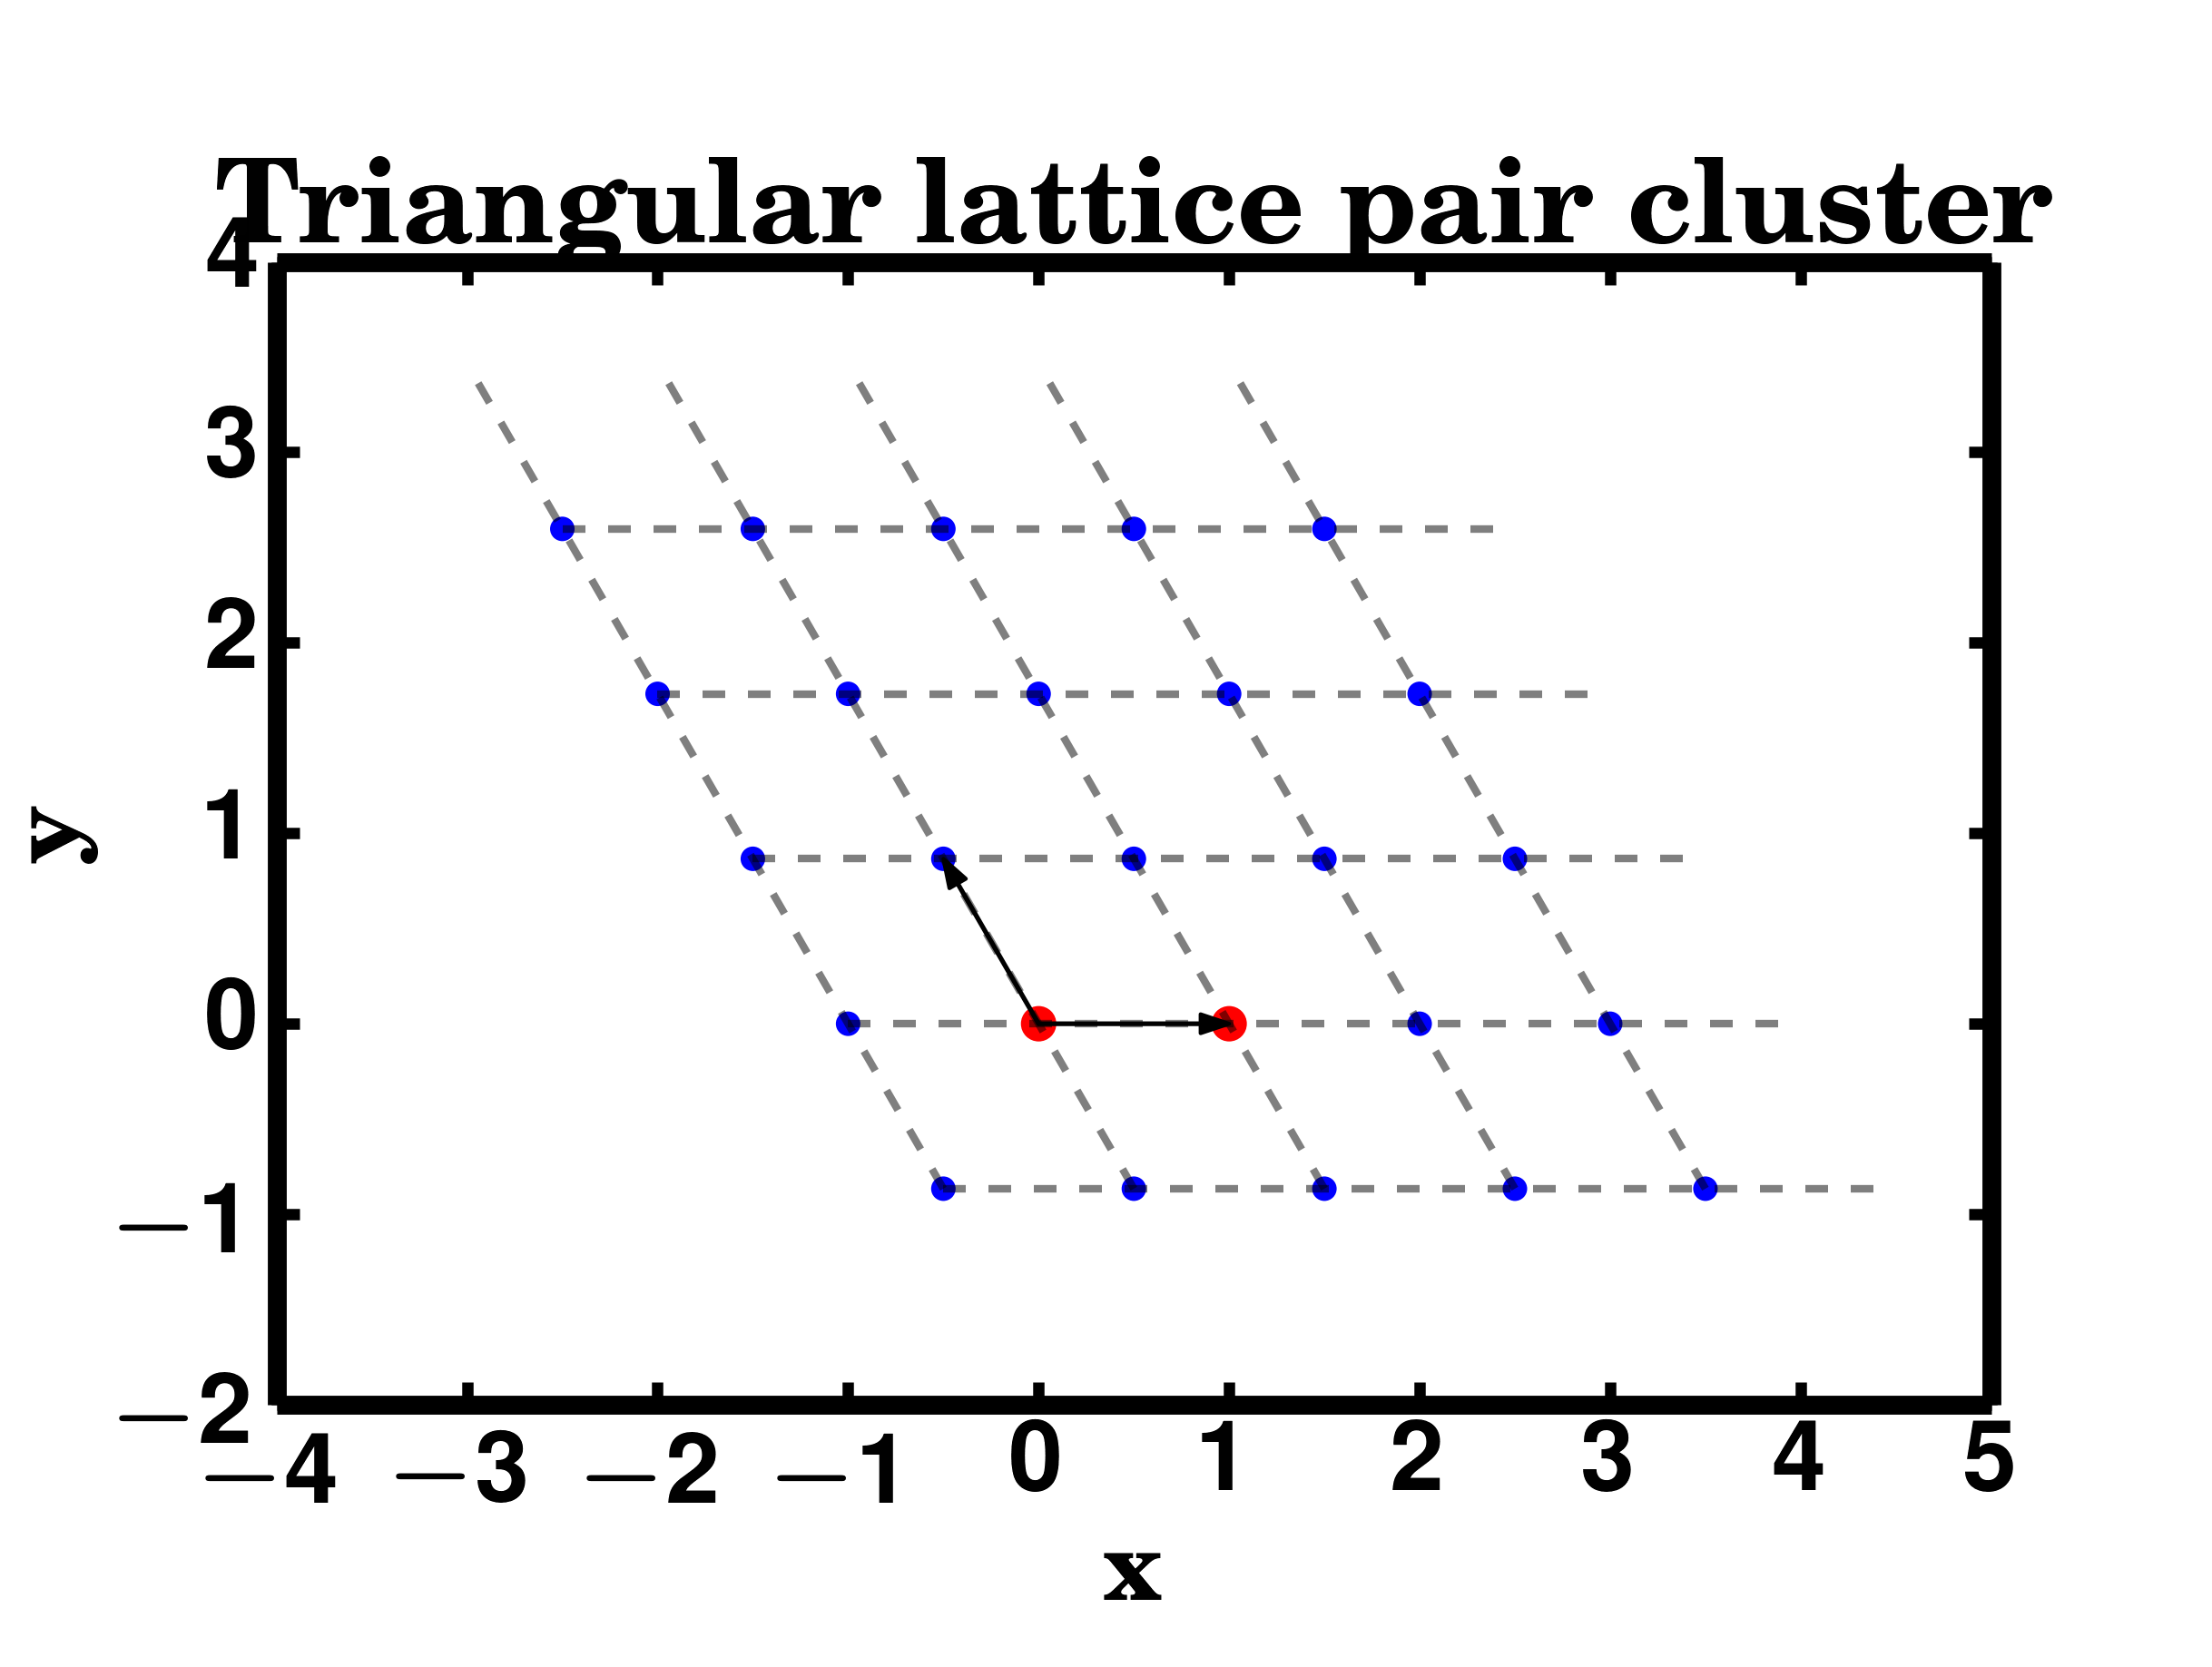
\includegraphics[max width=\textwidth]{./triangularclust.png}
    \end{center}
    \caption{Selected pair cluster (red) in a triangular lattice.}
    \label{fig:triangular}
\end{figure}

\begin{equation}
    \label{tensorbasis}
    \Phi=\Phi_{xx}\Lambda_{xx}+\Phi_{xy}\Lambda_{xy}+\Phi_{yx}\Lambda_{yx}+\Phi_{yy}\Lambda_{yy}
\end{equation}

Where $\Phi$ is the force constant matrix for the particular pair we're looking at
and $\Lambda$ is the appropriate starting tensor basis that reconstruct $\Phi$.

There is a total of 4 symmetry operations that leave the cluster invariant. Two of them
map the sites back onto themselves, while the other two result in the sites exchanging places.

\noindent
The following operations map the cluster sites onto themselves:

I0
\begin{equation}
    S=
    \begin{pmatrix}
        1.0&0.0\\
        0.0&1.0
    \end{pmatrix}
    ,\vec{\tau}=
    \begin{pmatrix}
        0.0\\
        0.0
    \end{pmatrix}
    \label{I0}
\end{equation}

M0
\begin{equation}
    S=
    \begin{pmatrix}
        1.0&0.0\\
        0.0&-1.0
    \end{pmatrix}
    ,\vec{\tau}=
    \begin{pmatrix}
        0.0\\
        0.0
    \end{pmatrix}
    \label{M0}
\end{equation}

\noindent
The following operations map the cluster sites onto each other:

R180
\begin{equation}
    S=
    \begin{pmatrix}
        -1.0&0.0\\
        0.0&-1.0
    \end{pmatrix}
    ,\vec{\tau}=
    \begin{pmatrix}
        1.0\\
        0.0
    \end{pmatrix}
    \label{R180}
\end{equation}

M90
\begin{equation}
    S=
    \begin{pmatrix}
        -1.0&0.0\\
        0.0&1.0
    \end{pmatrix}
    ,\vec{\tau}=
    \begin{pmatrix}
        1.0\\
        0.0
    \end{pmatrix}
    \label{M90}
\end{equation}

We apply the Reynolds operator to each $\Lambda$ with the first set of symmetry operations,
and repeat the process on $\Lambda^{T}$ with the second set of operations. After applying
these operations and normalizing by number of operations, the tensor basis becomes:

\begin{equation}
    \Lambda_{xx}=
        \begin{pmatrix}
        1.0&0.0\\
        0.0&0.0
    \end{pmatrix}
    \label{symbasis}
\end{equation}

\begin{equation}
    \Lambda_{xy}=
        \begin{pmatrix}
        0.0&0.0\\
        0.0&0.0
    \end{pmatrix}
    \label{symbasis}
\end{equation}

\begin{equation}
    \Lambda_{yx}=
        \begin{pmatrix}
        0.0&0.0\\
        0.0&0.0
    \end{pmatrix}
    \label{symbasis}
\end{equation}

\begin{equation}
    \Lambda_{yy}=
        \begin{pmatrix}
        0.0&0.0\\
        0.0&1.0
    \end{pmatrix}
    \label{symbasis}
\end{equation}

A QR decomposition (or simple observation in this case) reveals that only $\Lambda_{xx}$ and $\Lambda_{yy}$ are
needed to form the tensor basis, since the other two values are linearly dependent.

\section{Honeycomb structure: nearest neighbor tensor basis}
The process can be repeated for the nearest neighbor pair in a honeycomb structure.

\begin{figure}[h]
    \begin{center}
        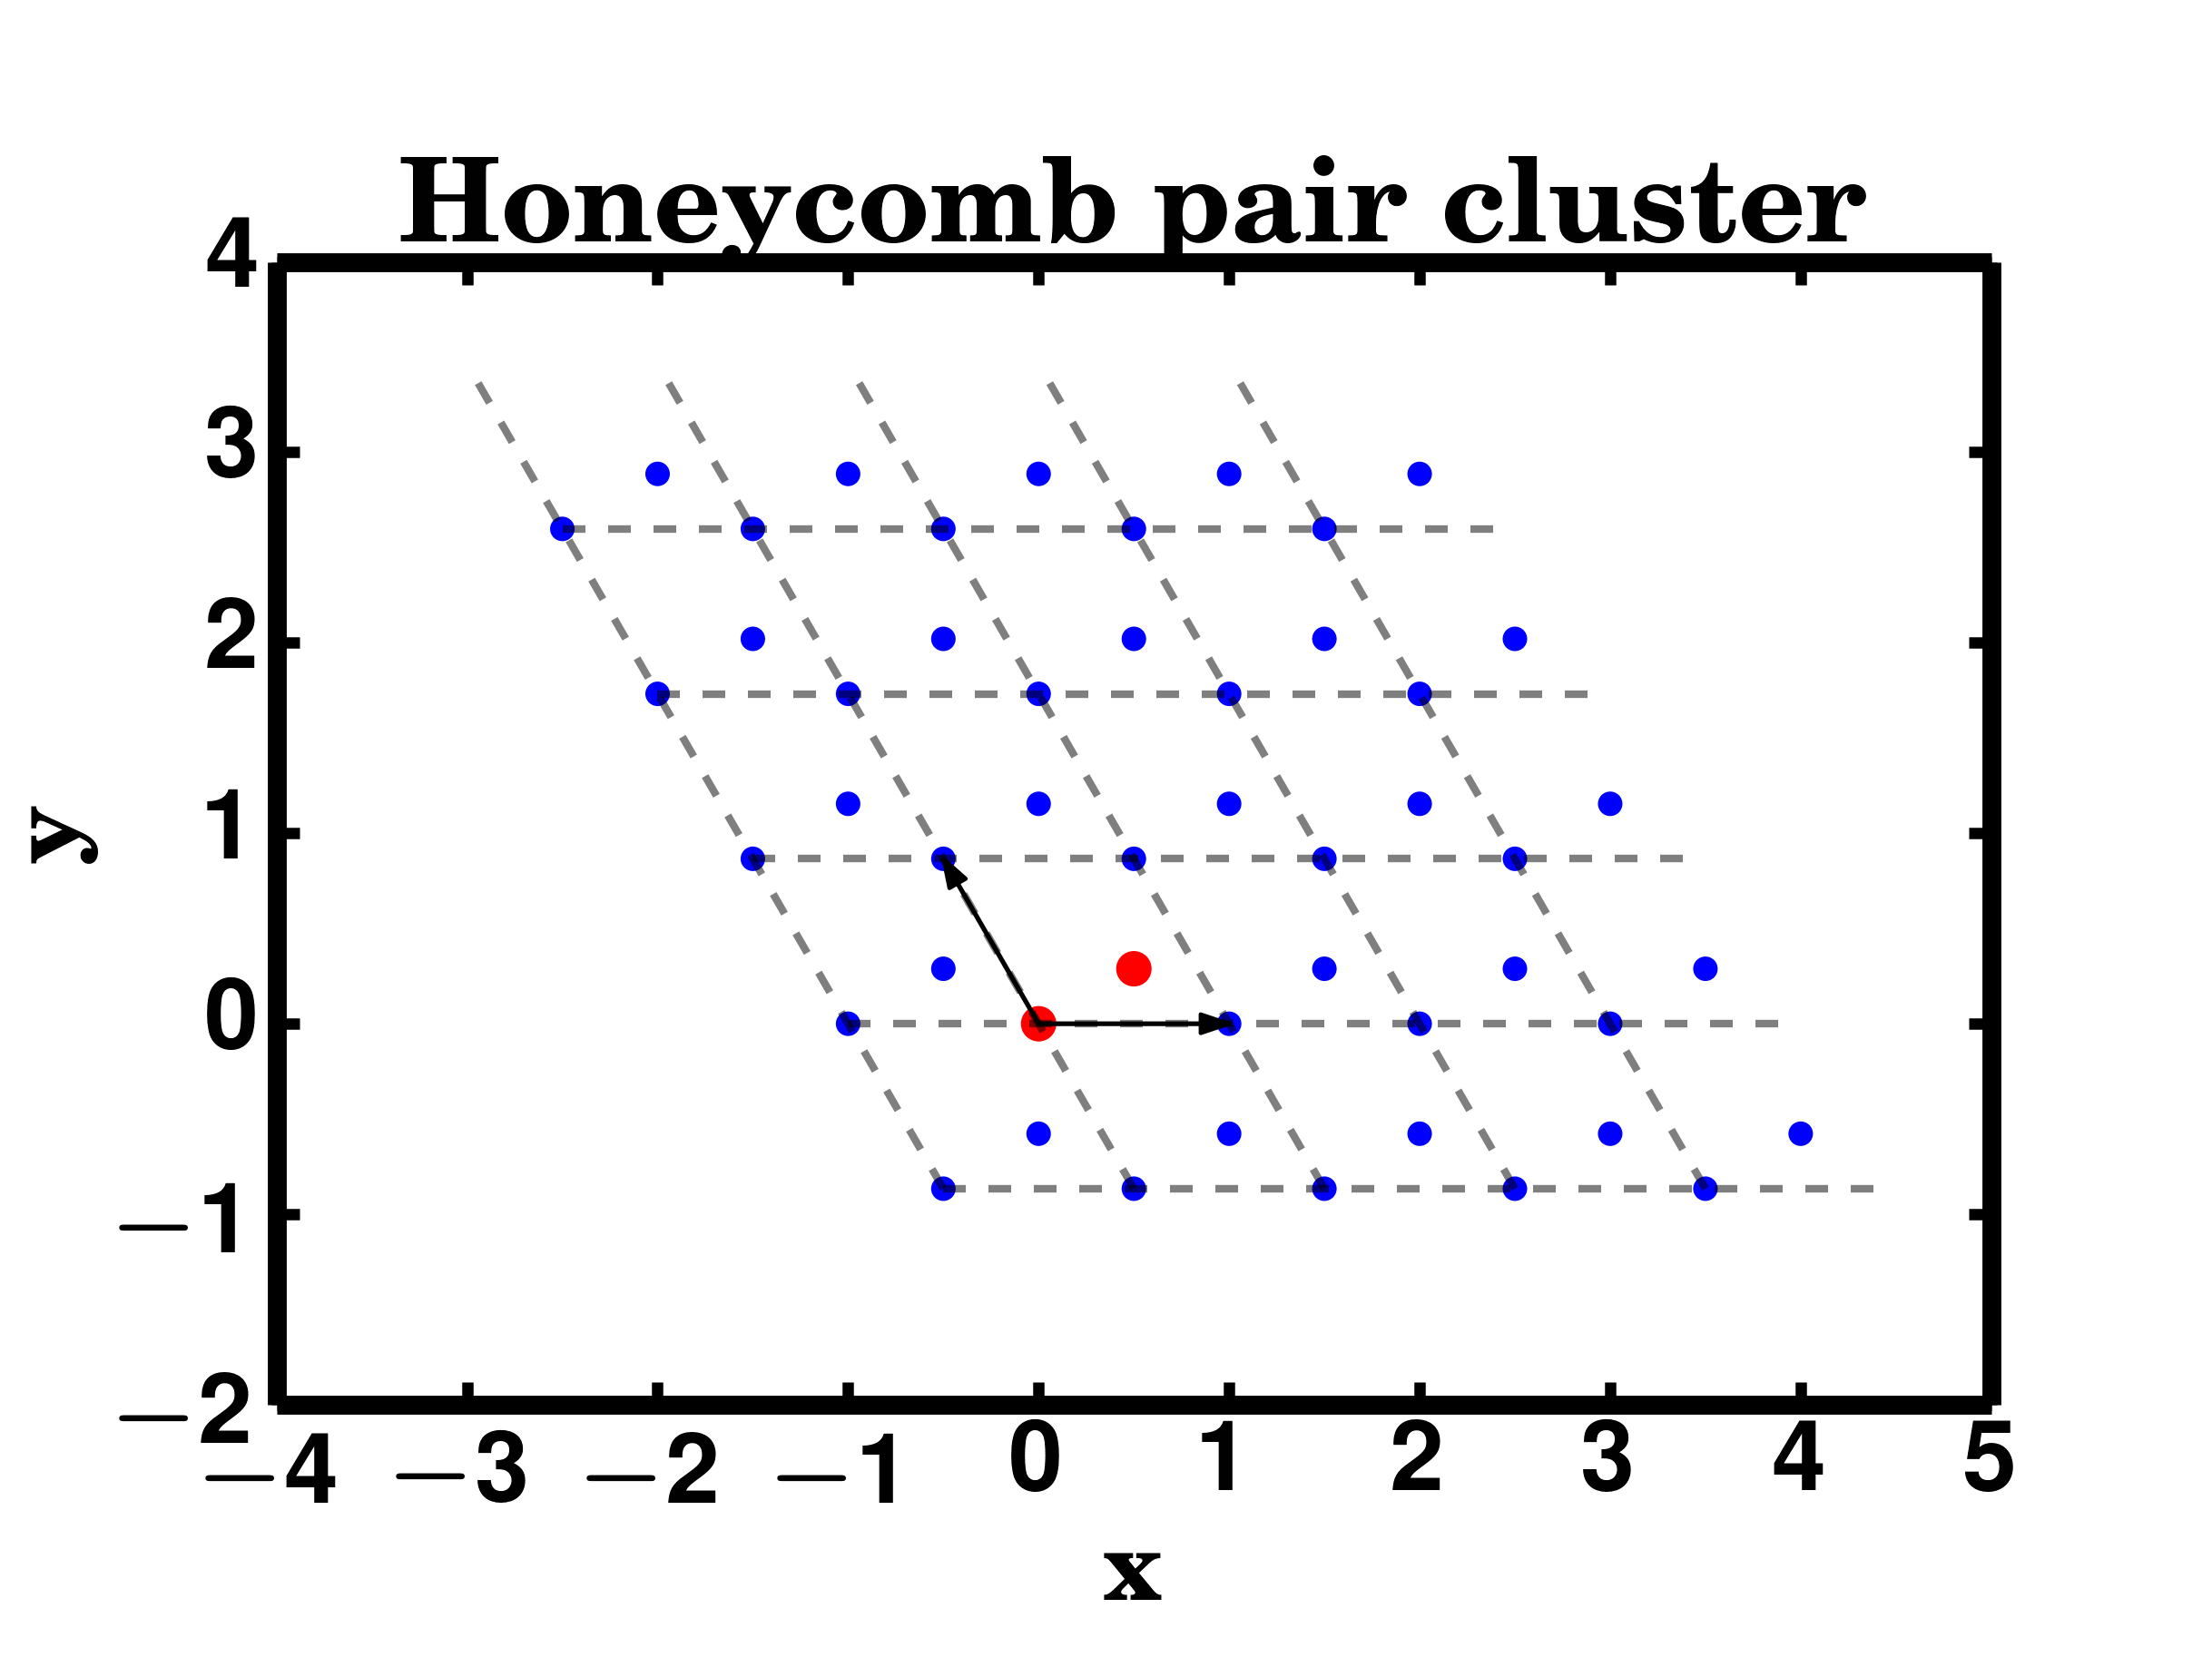
\includegraphics[max width=\textwidth]{./honeyclust.png}
    \end{center}
    \caption{Selected pair cluster (red) in a triangular lattice.}
    \label{fig:honeyclust}
\end{figure}

There is a total of 4 symmetry operations that leave the cluster invariant. Two of them
map the sites back onto themselves, while the other two result in the sites exchanging places.

\noindent
The following operations map the cluster sites onto themselves:

I0
\begin{equation}
    S=
    \begin{pmatrix}
        1.0&0.0\\
        0.0&1.0
    \end{pmatrix}
    ,\vec{\tau}=
    \begin{pmatrix}
        0.0\\
        0.0
    \end{pmatrix}
    \label{I0}
\end{equation}

M30
\begin{equation}
    S=
    \begin{pmatrix}
        0.5&\frac{\sqrt{3}}{2}\\
        \frac{\sqrt{3}}{2}&-0.5
    \end{pmatrix}
    ,\vec{\tau}=
    \begin{pmatrix}
        0.0\\
        0.0
    \end{pmatrix}
    \label{M30}
\end{equation}

\noindent
The following operations map the cluster sites onto each other:

R180
\begin{equation}
    S=
    \begin{pmatrix}
        -1.0&0.0\\
        0.0&-1.0
    \end{pmatrix}
    ,\vec{\tau}=
    \begin{pmatrix}
        0.5\\
        \frac{\sqrt{3}}{6}
    \end{pmatrix}
    \label{R180}
\end{equation}

M120
\begin{equation}
    S=
    \begin{pmatrix}
        -0.5&-\frac{\sqrt{3}}{2}\\
        -\frac{\sqrt{3}}{2}&0.5
    \end{pmatrix}
    ,\vec{\tau}=
    \begin{pmatrix}
        0.5\\
        \frac{\sqrt{3}}{6}
    \end{pmatrix}
    \label{M120}
\end{equation}

We apply the Reynolds operator to each $\Lambda$ with the first set of symmetry operations,
and repeat the process on $\Lambda^{T}$ with the second set of operations. After applying
these operations and normalizing by number of operations, the tensor basis becomes:

\begin{equation}
    \Lambda_{xx}=
    \begin{pmatrix}
        \frac{5}{8}&\frac{\sqrt{3}}{8}\\
        \frac{\sqrt{3}}{8}&\frac{3}{8}
    \end{pmatrix}
    \label{symbasis}
\end{equation}

\begin{equation}
    \Lambda_{xy}=
    \begin{pmatrix}
        \frac{\sqrt{3}}{8}&\frac{3}{8}\\
        \frac{3}{8}&-\frac{\sqrt{3}}{8}
    \end{pmatrix}
    \label{symbasis}
\end{equation}

\begin{equation}
    \Lambda_{yx}=
    \begin{pmatrix}
        \frac{\sqrt{3}}{8}&\frac{3}{8}\\
        \frac{3}{8}&-\frac{\sqrt{3}}{8}
    \end{pmatrix}
    \label{symbasis}
\end{equation}

\begin{equation}
    \Lambda_{yy}=
    \begin{pmatrix}
        \frac{3}{8}&-\frac{\sqrt{3}}{8}\\
        -\frac{\sqrt{3}}{8}&\frac{5}{8}
    \end{pmatrix}
    \label{symbasis}
\end{equation}

A QR decomposition reveals that only $\Lambda_{xx}$ and $\Lambda_{xy}$ are
needed to form the tensor basis, since the other two values are linearly dependent.
\end{document}
